\documentclass[PI,LAB]{HSEUniversity}

\usepackage{graphicx}
\graphicspath{ {img/} }

\usepackage{hyperref}
\hypersetup{
    colorlinks=true,
    linkcolor=black,
    filecolor=magenta,      
    urlcolor=cyan,
}

\title{Организация паттернов проектирования. Поведенческий паттерн <<Наблюдатель>>}
\author{Рязанов Иван Дмитриевич}
\supervisor{к.т.н., доцент кафедры Информационных технологий в бизнесе НИУ ВШЭ-Пермь}{А.В.~Кычкин}
\Year{2020}

\begin{document}
\maketitle
\chapter{Паттерн <<Наблюдатель>>}
\textbf{Название и классификация паттерна}

Наблюдатель – поведенческий паттерн, который реализует у класса механизм, позволяющий объекту этого класса получать оповещения об изменении состояния других объектов, и тем самым наблюдать за ними.

\textbf{Назначение}


\begin{enumerate}
  \item Паттерн Observer определяет зависимость "один-ко-многим" между объектами так, что при изменении состояния одного объекта все зависящие от него объекты уведомляются и обновляются автоматически. 
  \item Паттерн Observer инкапсулирует главный (независимый) компонент в абстракцию Subject и изменяемые (зависимые) компоненты в иерархию Observer. 
  \item Паттерн Observer определяет часть "View" в модели Model-View-Controller (MVC).   
\end{enumerate}

\textbf{Применимость}

Наблюдатель следует использовать, когда:
\begin{enumerate}
  \item существует, как минимум, один объект, рассылающий сообщения;
  \item имеется не менее одного получателя сообщений, причём их количество и состав могут изменяться во время работы приложения; 
  \item у абстракции есть два аспекта, один из которых зависит от другого. Инкапсуляции этих аспектов в разные объекты позволяют изменять и повторно использовать их независимо;
  \item при модификации одного объекта требуется изменить другие и заранее неизвестно, сколько именно объектов нужно изменить;
  \item один объект должен оповещать других, не делая предположений об уведомляемых объектах. Другими словами, вы не хотите, чтобы объекты были тесно связаны между собой.
\end{enumerate}

Данный шаблон часто применяют в ситуациях, в которых отправителя сообщений не интересует, что делают получатели с предоставленной им информацией.
Паттерн Observer находит широкое применение в системах пользовательского интерфейса, в которых данные и их представления ("виды") отделены друг от друга. При изменении данных должны быть изменены все представления этих данных (например, в виде таблицы, графика и диаграммы).

%\clearpage

\begin{figure}[h]
  \centering
  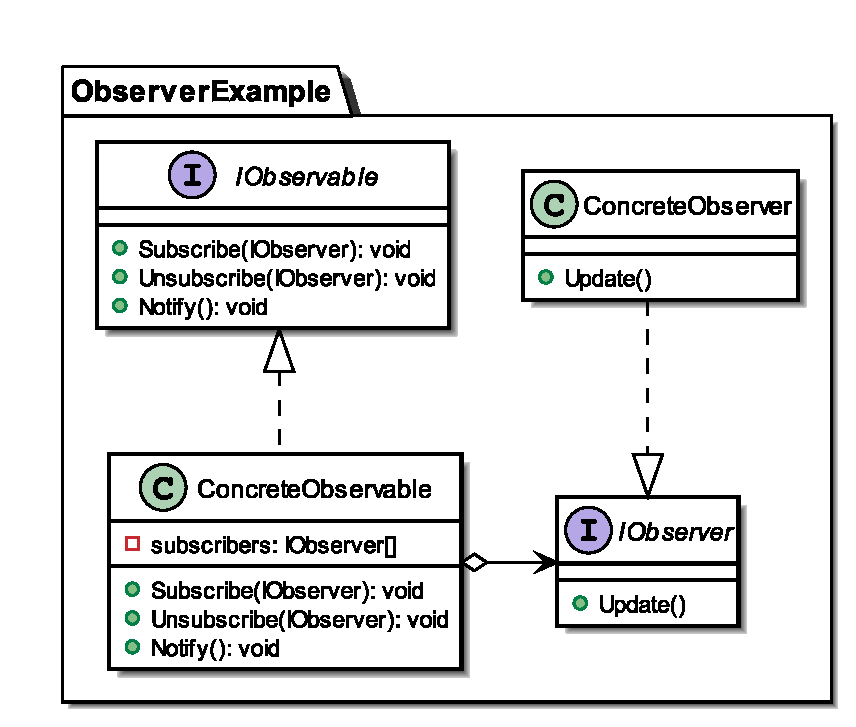
\includegraphics[scale=0.7]{Observer_CD.eps}
  \caption{Диаграмма классов паттерна <<Наблюдатель>>}
\end{figure}

\begin{figure}[h]
  \centering
  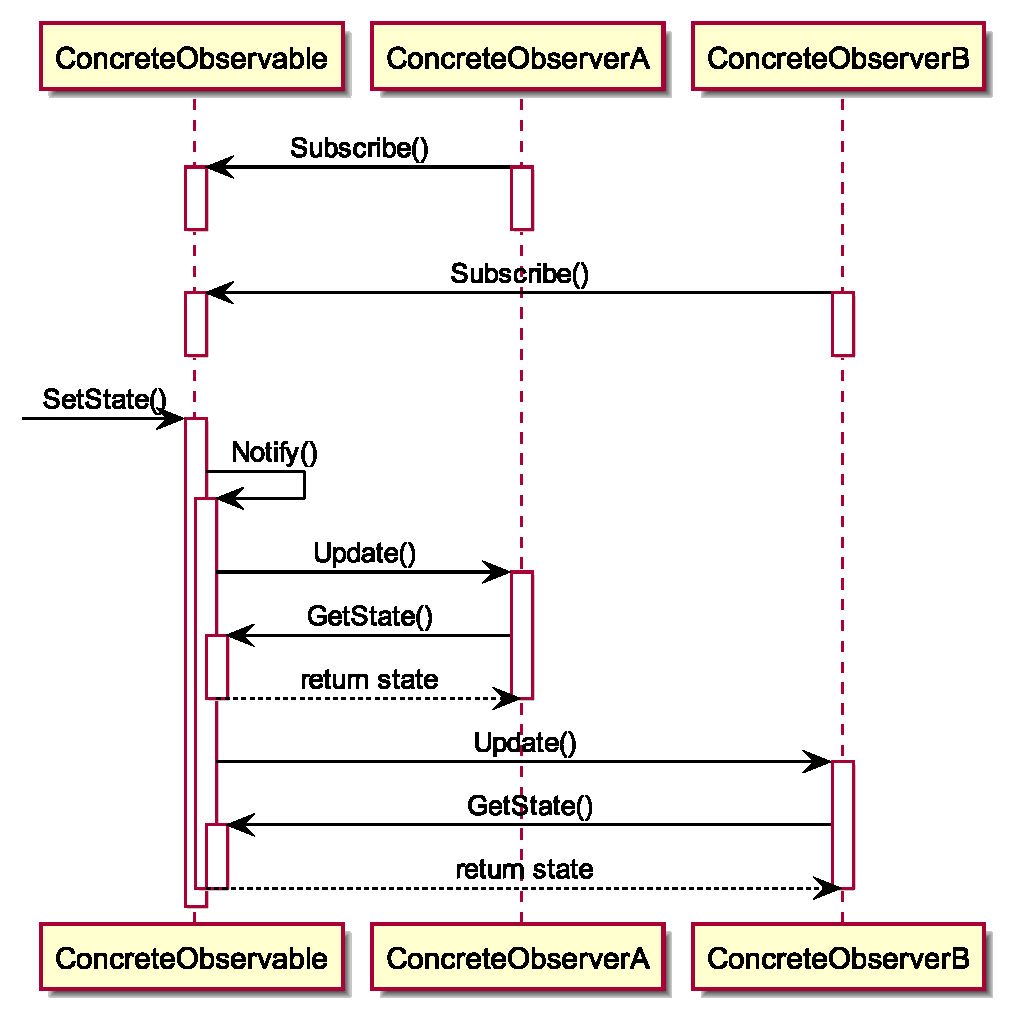
\includegraphics[scale=0.5]{Observer_SD.eps}
  \caption{Диаграмма последовательности паттерна <<Наблюдатель>>}
\end{figure}
\clearpage

\textbf{Участники}

\begin{enumerate}
  \item \code{IObservable}: представляет наблюдаемый объект (издатель). Определяет три метода: \code{Subscribe()} (для добавления наблюдателя), \code{Unsubscribe()} (удаление наблюдателя) и \code{Notify()} (уведомление наблюдателей)
  \item \code{ConcreteObservable}: конкретная реализация интерфейса \code{IObservable}. Определяет коллекцию объектов наблюдателей.
  \item \code{IObserver}: представляет наблюдателя (подписчика), который подписывается на все уведомления наблюдаемого объекта. Определяет метод \code{Update()}, который вызывается наблюдаемым объектом для уведомления наблюдателя.
  \item \code{ConcreteObserver}: конкретная реализация интерфейса \code{IObserver}.
\end{enumerate}

\textbf{Плюсы и минусы}

Плюсы:
\begin{enumerate}
	\item Издатели не зависят от конкретных классов подписчиков и наоборот.
  \item Вы можете подписывать и отписывать получателей на лету.
  \item Реализует принцип открытости/закрытости (SOLID).
\end{enumerate}

Минусы:
\begin{enumerate}
	\item Подписчики оповещаются в случайном порядке.
\end{enumerate}

\textbf{Области применения}

\begin{enumerate}
	\item Системы, обрабатывающие случайно приходящие события.
	\item Графические интерфейсы.
\end{enumerate}

\chapter{Проектирование и реализация}
\section{Проектирование}

Для разработки был выбран 1 вариант:

<<Программа для учета успеваемости студентов>>.

Перед началом работы построим диаграмму классов (см.~рис.~\ref{fig:Task_CD}).

\begin{figure}[h]
  \centering
  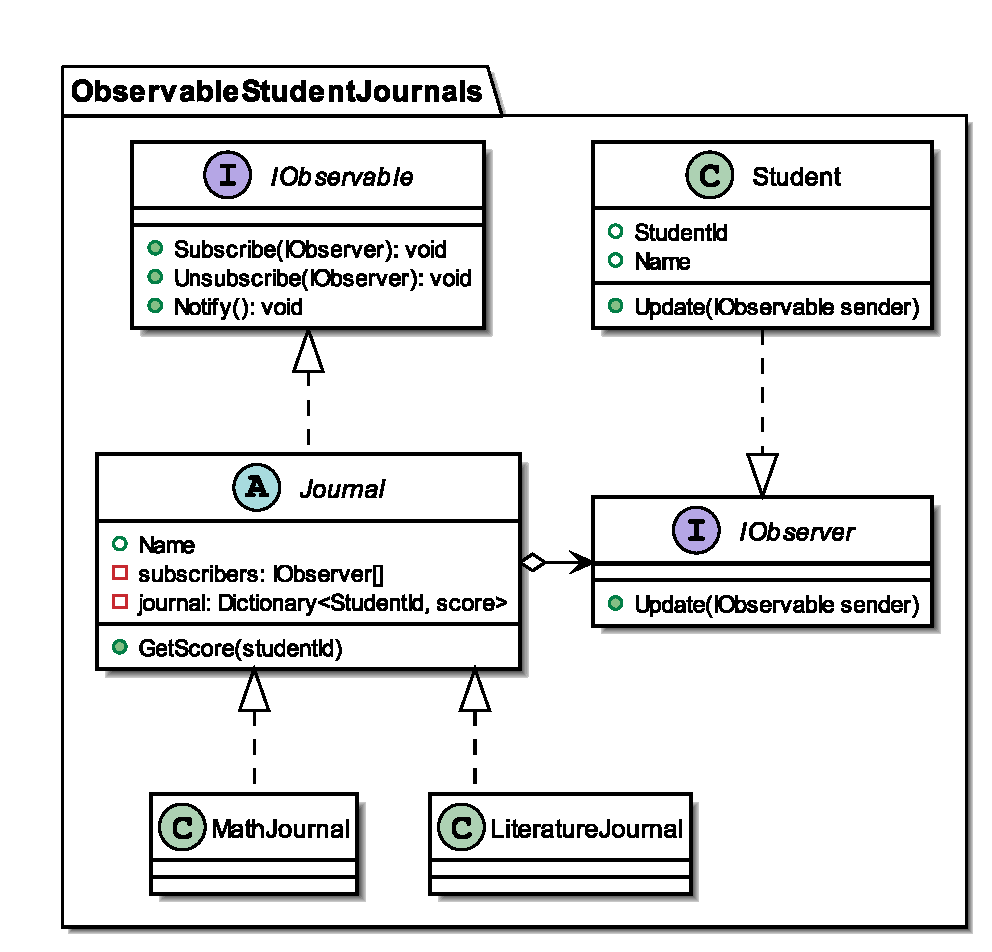
\includegraphics[scale=0.75]{Task_CD.eps}
  \caption{Диаграмма классов}
  \label{fig:Task_CD}
\end{figure}

\textbf{Участники}

\begin{enumerate}
  \item \code{IObservable}: представляет наблюдаемый объект (издатель). 
  \item \code{Journal}: конкретная реализация интерфейса \code{IObservable}. Абстрактный класс, определяющий список студентов, подписанных на изменения в журнале, сам журнал в виде словаря (ключ --- ID студента, значение --- оценка по предмету) и метод \code{GetScore(studentId)} для получения оценки по ID студента.
  \item \code{MathJournal}, \code{LiteratureJournal}: журналы оценок по математике и литературе.
  \item \code{IObserver}: представляет наблюдателя (подписчика), который подписывается на все уведомления наблюдаемого объекта.
  \item \code{Student}: конкретная реализация интерфейса \code{IObserver}. Студент, отслеживающий оценки.
\end{enumerate}

\section{Реализация}
Реализация паттерна <<Наблюдатель>> находится в git-репозитории по ссылке: \href{https://github.com/rovany706/design-patterns/tree/master/Observer/ObservableStudentJournals}{github.com}

\end{document}
